\documentclass[border=0pt]{standalone}

\def\xcolorversion{2.00}
\usepackage[dvipsnames]{xcolor}
\usepackage[utf8]{inputenc} 
\usepackage{amssymb,amsmath}


\usepackage{tikz}
\usetikzlibrary{arrows,%
                shapes,positioning,
                decorations.text,decorations.pathreplacing}
                
\thispagestyle{empty}
\begin{document}

\definecolor{lightgreen}{rgb}{0.56, 0.93, 0.56}
  
%\begin{center}
%\hspace{-2cm}
\begin{tikzpicture}[node distance   = 1.5 cm]
\centering
%  %\useasboundingbox (-1,-1) rectangle (11,11); 
%  \tikzset{VertexStyle/.style = {shape          = rectangle,
%  								draw, red, 
%  								line width=1pt, 
%                                 text           = black,
%                                 inner sep      = 2pt,
%                                 outer sep      = 0pt,
%                                 minimum size   = 4 pt}}
%  \tikzset{EdgeStyle/.style   = {thick,
%                                 double          = black,%yellow,
%                                 double distance = 1pt}}
%  \tikzset{LabelStyle/.style =   {draw,
%  								shape=circle, 
%                                  inner sep      = 1pt,
%                                 outer sep      = 0pt,
%                                  fill           = yellow,
%                                  text           = black}}
%  \tikzset{LabelStyle2/.style =   {draw,
%  								shape=circle, 
%                                  inner sep      = 1pt,
%                                 outer sep      = 0pt,
%                                  fill           = lightgreen,
%                                  text           = black}}
%
%     % n=0
%     \node[VertexStyle](A){$\varnothing$};
%     % n=1
%     \node[VertexStyle, below left=of A](B1){$v_0=1$};
%     \draw[EdgeStyle](A) to node{} (B1) ;
%     \node[VertexStyle, below right=of A](B2){$v_0=2$};
%     \draw[EdgeStyle, double=blue, double distance=2pt](A) to (B2);
%     % n=2
%     \node[VertexStyle, below=of B1](C1){$v_{-1}=1$};
%     \draw[EdgeStyle](C1) to node[LabelStyle]{$0$} (B1); 
%     \node[VertexStyle, below=of B2](C2){$v_{-1}=2$};
%     \draw[EdgeStyle](C2) to node[LabelStyle]{$0$} (B1); 
%     \draw[EdgeStyle, double=blue, double distance=2pt](C2) to node[LabelStyle]{$1$}  (B2); 
%     % n=3
%     \node[VertexStyle, below=of C1](D1){$v_{-2}=1$};
%     \draw[EdgeStyle](D1) to node[LabelStyle2]{$1$} (C1); 
%     \node[VertexStyle, below=of C2](D2){$v_{-2}=2$};
%     \draw[EdgeStyle, double=blue, double distance=2pt](D1) to node[LabelStyle2]{$0$} (C2); 
%     \draw[EdgeStyle](D2) to node[LabelStyle2]{$0$} (C2); 


%%%% CUTTING STACKING 0 %%%
%\node[right=of A](cs0)
%{
%\begin{tikzpicture}
%  \tikzset{VertexStyle/.style = {shape          = rectangle,
%  								draw, red, 
%  								line width=1pt, 
%                                 text           = black,
%                                 inner sep      = 2pt,
%                                 outer sep      = 2pt,
%                                 minimum size   = 4 pt}}
%    \begin{scope}[every label/.style={inner sep=5pt, draw=none,rectangle,fill=none}, every node/.style={fill=black,circle,inner sep=0pt,minimum size=5pt}, blabel/.style={label={above:#1}}, bblabel/.style 2 args={label={[label distance=#2, VertexStyle]below:#1}}, alabel/.style={label={above:#1}}]
%	%%% TOUR DE GAUCHE %%%
%    \tikzset{node distance = 3 cm}
%	\node[blabel={$0$}{}](a){};
%	\node[right=of a, blabel={$1$}](b){};
%	\draw(a) to node[bblabel={$\varnothing$}{0pt}, draw=none, fill=none]{} (b) ;
%	\node[right=2.7cm of a, label={[blue, inner sep=3pt]above:$\gamma$}, fill=blue](x){};
%  \end{scope}
%\end{tikzpicture}
%};


%%% CUTTING STACKING 1 %%%
\node (cs1) % at ([shift=({-100pt,20pt})]B1)
{
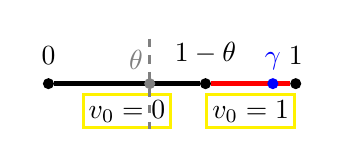
\begin{tikzpicture}
  \tikzset{VertexStyle/.style = {shape          = rectangle,
  								draw, yellow, 
  								line width=1pt, 
                                 text           = black,
                                 inner sep      = 2pt,
                                 outer sep      = 2pt,
                                 minimum size   = 4 pt}}
    \begin{scope}[every label/.style={inner sep=5pt, draw=none,rectangle,fill=none}, every node/.style={fill=black,circle,inner sep=0pt, outer sep=0pt, minimum size=4pt}, blabel/.style={label={above:#1}}, bblabel/.style 2 args={label={[label distance=#2, VertexStyle]below:#1}}, alabel/.style={label={above:#1}}, line width=2pt]
	%%% TOUR DE GAUCHE %%%
%    \tikzset{node distance = 3 cm}
	\node[blabel={$0$}{}](a){};
	\node[right=1.854102cm of a, blabel={$1-\theta$}](b){};
	\draw(a) to node[bblabel={$v_0=0$}{0pt}, draw=none, rectangle, fill=none]{} (b);
%	\draw(a) to  (b);
	%%% TOUR DE DROITE %%%
	%
%	\tikzset{node distance = 1 cm};
	\node[right=3cm of a, blabel={$1$}](c){};
	%
	\draw[draw=red] (b) to node[bblabel={$v_0=1$}{0pt}, draw=none, rectangle, fill=none]{} (c);
%	\draw[draw=red] (b) to (c);
	\node[left=0.15cm of c, label={[blue, inner sep=3pt]above:$\gamma$}, fill=blue](x){};
%% DÉCOUPAGE
	\node[right=1.145898cm of a, label={[gray, inner sep=3pt, xshift=-5pt]above:$\theta$}, fill=gray](theta){};
	\node[above=0.5cm of theta, draw=none, fill=none](U){};
	\node[below=0.5cm of theta, draw=none, fill=none](L){};
	\draw[line width=1pt, draw=gray, dashed](U) to (L);
  \end{scope}
\end{tikzpicture}
};

%%% CUTTING STACKING 2 %%%
\node[below=0.1cm of cs1](cs2)
{
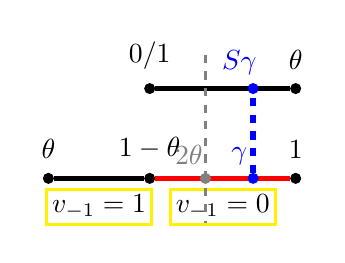
\begin{tikzpicture}
  \tikzset{VertexStyle/.style = {shape          = rectangle,
  								draw, yellow, 
  								line width=1pt, 
                                 text           = black,
                                 inner sep      = 2pt,
                                 outer sep      = 2pt,
                                 minimum size   = 4 pt}}
  \tikzset{EpsilonStyle/.style = {shape          = circle,
                                 text           = black,
                                 minimum size   = 15 pt,
                                 line width = 0.75pt, fill=yellow, draw=black, scale=0.8}}
    \begin{scope}[every label/.style={inner sep=5pt, draw=none,rectangle,fill=none}, every node/.style={fill=black,circle,inner sep=0pt,outer sep=0pt, minimum size=4pt}, bblabel/.style 2 args={label={[label distance=#2, VertexStyle]below:#1}}, blabel/.style={label={above:#1}}, line width=2pt]
	%%% TOUR DE GAUCHE %%%
%    \tikzset{node distance = 1 cm}
	\node[blabel={$\theta$}{}](a){};
	\node[right=1.145898cm of a, blabel={$1-\theta$}](b){};
	\draw(a) to node[bblabel={$v_{-1}=1$}{0pt}, draw=none, rectangle, fill=none]{} (b);
%	\draw(a) to  (b);
		%%% TOUR DE DROITE %%%
	%
%	\tikzset{node distance = 1 cm};
	\node[above=1cm of b, blabel={$0/1$}](b1){};
	%
%	\tikzset{node distance = 3 cm};
	\node[right=3cm of a, blabel={$1$}](c){};
	%
	\tikzset{node distance = 1 cm};
	\node[above=of c, blabel={$\theta$}](c1){};
	\draw[draw=red](b) to node[bblabel={$v_{-1}=0$}{0pt}, draw=none, rectangle, fill=none]{} (c);
%	\draw[draw=red](b) to (c);
	\draw(b1) to (c1);
	% 
%	\node[right=5pt of c, EpsilonStyle](){$1$};
%	\node[right=5pt of c1, EpsilonStyle](){$0$};
	%%% CLASSE DE x %%%
	%
	\node[distance=0.5cm, left=0.4cm of c, fill=blue, label={[blue, inner sep=3pt, xshift=-5pt]above:$\gamma$}](x){};
	%
	\node[above=of x, label={[blue, inner sep=3pt, xshift=-5pt]above:$S\gamma$}, fill=blue](x1){};
	\draw[blue, dashed](x) to (x1);
%% DÉCOUPAGE
	\node[right=1.854102cm of a, label={[gray, inner sep=3pt, xshift=-6pt]above:$2\theta$}, fill=gray](theta){};
	\node[above=1.5cm of theta, draw=none, fill=none](U){};
	\node[below=0.5cm of theta, draw=none, fill=none](L){};
	\draw[line width=1pt, draw=gray, dashed](U) to (L);
	
  \end{scope}
\end{tikzpicture}
};

%%% CUTTING STACKING 3 %%%
%\node[below=-20pt of cs1](cs3)
\node[below=0.1cm of cs2, xshift=-3pt] (cs3) %at ([shift=({30pt,-150pt})]cs1)
{
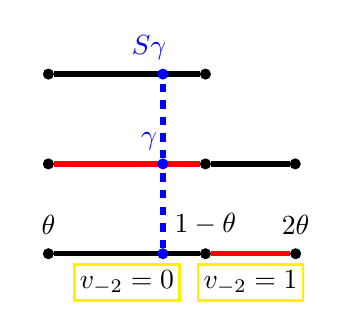
\begin{tikzpicture}
  \tikzset{VertexStyle/.style = {shape          = rectangle,
  								draw, yellow, 
  								line width=1pt, 
                                 text           = black,
                                 inner sep      = 2pt,
                                 outer sep      = 2pt,
                                 minimum size   = 4 pt}}
  \tikzset{EpsilonStyle/.style = {shape          = circle,
                                 text           = black,
                                 minimum size   = 15 pt,
                                 line width = 1pt, fill=lightgreen, draw=black}}
	\scalebox{1}{
  \begin{scope}[every label/.style={inner sep=5pt, draw=none,rectangle,fill=none}, every node/.style={fill=black,circle,inner sep=0pt,outer sep=0pt, minimum size=4pt}, bblabel/.style 2 args={label={[label distance=#2, VertexStyle]below:#1}}, blabel/.style={label={above:#1}}, line width=2pt]
	%%% TOUR DE GAUCHE %%%
%    \tikzset{node distance = 2 cm}
	\node[blabel={$\theta$}{}](a){};
	\node[right=1.854102cm of a, blabel={$1-\theta$}](b){};
	\draw(a) to node[bblabel={$v_{-2}=0$}{0pt}, draw=none, rectangle, fill=none]{} (b);
%	\draw(a) to (b);
	\tikzset{node distance = 1 cm}
	\node[above=of a](a1){};
	\node[above=of a1](a2){};
	\node[above=of b](b1){};
	\node[above=of b1](b2){};
	\draw[draw=red](a1) to (b1);
	\draw(a2) to (b2);
	%%% TOUR DE DROITE %%%
	%
	\tikzset{node distance = 1 cm};
	\node[right=3cm of a, blabel={$2\theta$}](c){};
	\node[right=of b1](c1){};
	\draw[draw=red](b) to node[bblabel={$v_{-2}=1$}{0pt}, draw=none, rectangle, fill=none]{} (c);
%	\draw[draw=red](b) to  (c);
	\draw(b1) to (c1);
	%%% ORBITE %%%
	\node[distance=0.25cm, left=0.4cm of b, fill=blue](x){};
	\tikzset{node distance = 1 cm};
	\node[above=of x, fill=blue, label={[blue, inner sep=3pt, xshift=-5pt]above:{ $\gamma$}}](x1){};
	\node[above=of x1, fill=blue, label={[blue, inner sep=3pt, xshift=-5pt]above: $S\gamma$}](x2){};
	\draw[blue, dashed](x) to (x1);
	\draw[blue, dashed](x1) to (x2);
%	%% BRACES %%
%	\draw[decorate, decoration={brace,amplitude=10pt, raise=14pt}, blue, line width=2pt] ([yshift=-5pt]a1.west) -- ([yshift=5pt]a2.west)  node[midway, EpsilonStyle, xshift=-34pt]{$0$};
%	\node[node distance=3pt, above=of a, fill=none](ashiftdown){};
%	\node[node distance=3pt, below=of a, fill=none](ashiftup){};
%	\begin{pgflowlevelscope}{\pgftransformscale{2}}
%    		\draw[decorate, decoration={brace,amplitude=5pt, raise=6pt}, blue, line width=1pt] (ashiftup.west)--(ashiftdown.west) node[scale=0.5, midway, text=black, minimum size = 15pt, line width = 0.5pt, fill=lightgreen, draw=black, xshift=-32pt]{$1$};
%	\end{pgflowlevelscope}
%	\draw[decorate, decoration={brace,amplitude=10pt, raise=14pt, mirror}, blue, line width=2pt] ([yshift=-5pt]c.east) -- ([yshift=5pt]c1.east) node[midway, EpsilonStyle, xshift=34pt]{$0$};
  \end{scope}
}
\end{tikzpicture}
};

\node[right=0.3cm of cs1, scale=0.8](){$n=0$} ;
\node[right=0.3cm of cs2, scale=0.8](){$n=-1$} ;
\node[right=0.3cm of cs3, scale=0.8](){$n=-2$} ;

  \end{tikzpicture}
%\end{center}
\end{document}